\documentclass{article}
\usepackage[x11names, rgb]{xcolor}
\usepackage[utf8]{inputenc}
\usepackage{tikz}
\usetikzlibrary{snakes,arrows,shapes}
\usepackage{amsmath}
%
%

%

\usepackage{hyperref}
\usetikzlibrary{arrows,shapes,petri,external,arrows.meta}
	\tikzexternalize
	\tikzsetnextfilename{figure}
	\tikzset{
	place/.style={
	circle,
	thick,
	draw=black!100, % draw=blue!75,
    % fill=blue!20,
    minimum size=6mm
  },
  extPlace/.style={
    circle,
    dotted,
    draw=black!100, % draw=blue!75,
    % fill=blue!20,
    minimum size=6mm
  },
  extTransition/.style={
    rectangle,
    dotted,
    fill=white,
    minimum width=8mm,
    inner ysep=0.7pt
  },
  transition/.style={
    rectangle,
    thick,
    fill=black,
    minimum width=8mm,
    inner ysep=0.7pt
  },
  extTimedtransition/.style={
    rectangle,
    dotted,
    fill=white,
    minimum width=8mm,
    inner ysep=2pt
  },
  timedtransition/.style={
    rectangle,
    thick,
    fill=black,
    minimum width=8mm,
    inner ysep=2pt
  },
  inhibitor/.style={-o},
  text/.style={}
}%

\begin{document}
\pagestyle{empty}
%
%
%

\enlargethispage{100cm}
% Start of code
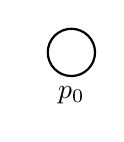
\begin{tikzpicture}[>=latex',line join=bevel,]
%%
\node (p0) at (27.0bp,18.0bp) [draw,ellipse,place, label=above:, label=left:$p_{0}$,rotate=90] {};
%
\end{tikzpicture}
% End of code

%
\end{document}
%



